\section{Motion Planning Using the Double Integrator Model} \label{sec:motion_planning_using_point_mass}

This section develops a motion planning framework using the double integrator model from \ref{subsec:point_mass_model}, transitioning from a global
coordinate representation to a Frenet frame formulation, as introduced in \ref{subsec:curve_following_coordinate_system}.
The Frenet frame provides a more structured approach for path tracking along a predefined road, accounting for curvature and alignment errors.
Our formulation builds on the work of Eilbrecht et al.
\cite{eilbrecht_challenges_2020} and systematically addresses motion dynamics, constraints, and control strategies.

\subsection{Overview of the Motion Planning Framework}

To effectively model and control vehicle motion, we employ a structured approach that systematically integrates kinematics, dynamics, constraints,
and control transformations.

We begin by defining the \textbf{coordinate transformation and kinematics}, introducing the curvature $C(s)$ of the reference path and the alignment
error $\xi = \psi - \theta$.
These definitions allow us to derive the first- and second-order kinematic equations, which describe how the vehicle's body-fixed velocity components
influence its evolution in Frenet coordinates.

Next, we formulate the \textbf{system dynamics} within the Frenet frame, defining the state vector and control inputs.
By incorporating the effects of curvature and alignment error, we capture both longitudinal and lateral dynamics within our model.

To address the nonlinearities introduced by the curvature terms, we employ \textbf{feedback linearization}.
This process involves assuming alignment to simplify the nonlinear dynamics, enabling the introduction of artificial control variables that linearize
the system.

To ensure that the planned trajectories remain within physical and operational limits, we carefully handle \textbf{constraint formulation}.
We derive bounds on velocity and acceleration and map them from the body-fixed frame to the Frenet frame, thereby enforcing vehicle and road
constraints within the planning model.

A key challenge in motion planning is the presence of \textbf{non-convexities} introduced by curvature-dependent constraints.
To address this, we use \textbf{quantifier elimination} techniques to obtain convex inner approximations of the feasible set.
We explore two approaches:
\begin{itemize}
	\item Interval Fitting, which provides a computationally efficient, box-shaped approximation of the constraint set.
	\item Cylindrical Algebraic Decomposition (CAD), a method from computer algebra that decomposes space into cylindrical cells to eliminate quantifiers while preserving logical equivalence.
\end{itemize}

Once an optimal trajectory is determined, we establish a \textbf{control transformation} that maps the optimized state and control variables to
physical vehicle inputs.
This step derives the necessary steering angle and longitudinal acceleration, ensuring compatibility with standard vehicle controllers.

Next, we provide the \textbf{exact discretization of the double integrator model}, ensuring an accurate transition from continuous to discrete-time
dynamics.
By leveraging matrix exponentials, this formulation preserves system behavior over discrete time steps.

Finally, we present the \textbf{complete motion planning model} as a formalized representation.
This encapsulates the system's state-space dynamics, control inputs, constraints, and transformation mappings.

\subsection{Coordinate Transformation and Kinematics}

In this subsection, we establish the foundation for our motion planning framework by describing the geometry of the reference path and deriving the
vehicle's kinematic equations in the Frenet frame.

First, let \(\theta(s)\) denote the tangent angle at an arc length \(s\) along the reference path.
The curvature, \(C(s)\), quantifies the rate of change of this tangent angle with respect to \(s\) and is defined as:
\begin{equation}
	C(s) := \frac{d\theta}{ds}.
\end{equation}

Next, consider the vehicle's orientation, \(\psi\).
To measure how much the vehicle deviates from following the road's direction, we define the alignment error \(\xi\) as:
\begin{equation}
	\xi := \psi - \theta.
\end{equation}
This error quantifies the difference between the vehicle's heading and the path's tangent direction.

Using these definitions and standard coordinate transformation techniques \cite{eilbrecht_challenges_2020}, we can derive the vehicle's motion
dynamics in the Frenet frame.
In this framework, the velocity components in the vehicle's body-fixed frame are directly related to the time derivatives of the Frenet coordinates.

\paragraph{First-Order Kinematics}\label{par:first_order_kinematics}
The following equations describe how the vehicle's position evolves along the path:
\begin{align}
	\dot{s}\,(1 - n\,C(s)) & = v_x\cos{\xi} - v_y\sin{\xi}, \label{eq:first_derivative_long} \\
	\dot{n}                & = v_x\sin{\xi} + v_y\cos{\xi}, \label{eq:first_derivative_lat}
\end{align}
where:
\begin{itemize}
	\item \(s\) is the longitudinal position along the reference path,
	\item \(n\) represents the lateral deviation from the path,
	\item \(v_x\) and \(v_y\) are the velocity components in the body-fixed frame.
\end{itemize}
Note that the term \(1 - n\,C(s)\) adjusts the longitudinal progress to account for the path's curvature.

\paragraph{Acceleration Dynamics}\label{par:acceleration_dynamics}
To capture the dynamics of acceleration in the Frenet frame, we introduce transformed acceleration components \(a_{x,tn}\) and \(a_{y,tn}\).
These dynamics are given by:
\begin{align}
	a_{x,tn} & = (a_x - v_y\,\dot{\psi})\cos{\xi} - (a_y + v_x\,\dot{\psi})\sin{\xi}, \label{eq:second_derivative_long} \\
	a_{y,tn} & = (a_x - v_y\,\dot{\psi})\sin{\xi} + (a_y + v_x\,\dot{\psi})\cos{\xi}, \label{eq:second_derivative_lat}
\end{align}
with the following definitions:
\begin{align}
	a_{x,tn} & := \ddot{s}\,(1 - n\,C(s)) - 2\dot{n}\,C(s)\dot{s} - n\,C'(s)\dot{s}^2, \label{def:axtn} \\
	a_{y,tn} & := \ddot{n} + C(s)\dot{s}^2\,(1 - n\,C(s)). \label{def:aytn}
\end{align}
These equations illustrate how the vehicle's acceleration in the Frenet frame is influenced by both its inherent dynamics (through \(\ddot{s}\) and
\(\ddot{n}\)) and the geometry of the reference path (through \(C(s)\) and its derivative \(C'(s)\)).

In summary, this subsection defines the key geometric parameters and derives the kinematic equations necessary for representing vehicle motion in the
Frenet frame.
These results set the stage for the subsequent development of the full motion planning model.

\subsection{System Dynamics Formulation}

We can now formalize the motion planning model in the Frenet frame by defining the state and control input vectors.
The state vector, denoted by \(x_{di}\), captures the vehicle's position, alignment error, and their corresponding velocities:
\begin{equation}
	x_{di} = \begin{bmatrix}
		s       \\
		n       \\
		\xi     \\
		\dot{s} \\
		\dot{n} \\
		\dot{\psi}
	\end{bmatrix},
\end{equation}
where:
\begin{itemize}
	\item \(s\) is the longitudinal position along the reference path,
	\item \(n\) is the lateral deviation,
	\item \(\xi\) is the alignment error (\(\psi - \theta\)),
	\item \(\dot{s}\), \(\dot{n}\), and \(\dot{\psi}\) are the corresponding time derivatives.
\end{itemize}

The control inputs are represented by the vector \(u_{di}\), which comprises the body-fixed accelerations:
\begin{equation}
	u_{di} = \begin{bmatrix}
		a_x \\
		a_y \\
		a_\psi
	\end{bmatrix}.
\end{equation}

Using the kinematic relationships derived earlier in \nameref{par:first_order_kinematics} and \nameref{par:acceleration_dynamics}, the dynamics of the double integrator model in the Frenet frame can be expressed as:
\begin{equation}
	\label{eq:frenet_frame_pm_dynamics_0}
	f_{di}(x_{di}, u_{di}) = \begin{bmatrix}
		\dot{s}                                                                                \\
		\dot{n}                                                                                \\
		\dot{\psi} - C(s)\dot{s}                                                               \\
		\displaystyle \frac{a_{x,tn} + 2\dot{n}\,C(s)\dot{s} + n\,C'(s)\dot{s}^2}{1 - n\,C(s)} \\
		a_{y,tn} - C(s)\dot{s}^2(1 - n\,C(s))                                                  \\
		a_\psi
	\end{bmatrix}.
\end{equation}

This formulation captures the vehicle's motion along a curved path by incorporating both its intrinsic dynamics and the influence of road curvature.
It is important to note that the curvature terms \(C(s)\) and \(C'(s)\) introduce non-convexities into the system dynamics.
We address these challenges in subsequent sections through feedback linearization.

\subsection{Linearization via Feedback Control} \label{subsec:constraints}
To simplify the nonlinear dynamics introduced by the curvature terms, we first decouple the body-fixed inputs in
\eqref{eq:frenet_frame_pm_dynamics_0}.
By substituting \eqref{eq:frenet_frame_pm_dynamics_0} the accelerations in the Frenet frame with their body-fixed relations from
\eqref{eq:second_derivative_long} and \eqref{eq:second_derivative_lat} in \eqref{eq:frenet_frame_pm_dynamics_0}, we obtain:
\begin{align}
	\frac{(a_x - v_y\,\dot{\psi})\cos{\xi} - (a_y + v_x\,\dot{\psi})\sin{\xi} + 2\dot{n}\,C(s)\dot{s} + n\,C'(s)\dot{s}^2}{1 - n\,C(s)} \\
	(a_x - v_y\,\dot{\psi})\sin{\xi} + (a_y + v_x\,\dot{\psi})\cos{\xi} - C(s)\dot{s}^2(1 - n\,C(s))
\end{align}
We observe that both entries contain the body-fixed control inputs \(a_x\) and \(a_y\).
To simplify the model, we make the following key assumption.

\subsubsection{Assumption: Alignment Error} \label{subsubsec:alignment_error}
We assume that the vehicle is always aligned with the road, i.e.,
\begin{equation}
	\xi = \psi - \theta = 0.
\end{equation}
This assumption leads to several useful simplifications:
\begin{itemize}
	\item The body-fixed accelerations are directly given by the transformed accelerations:
	      \[
		      [a_x,\, a_y] = [a_{x,tn},\, a_{y,tn}].
	      \]
	\item The rate of change of the vehicle's orientation becomes:
	      \[
		      \dot{\psi} = \dot{\theta} = C(s)\,\dot{s},
	      \]
	      where \(C(s)=\frac{d\theta}{ds}\).
	\item The yaw acceleration satisfies:
	      \[
		      a_\psi = \ddot{\psi} = \ddot{\theta} = C'(s)\,\dot{s}^2 + C(s)\,\ddot{s}.
	      \]
\end{itemize}
Although this assumption fixes the orientation to the road, the vehicle is still permitted lateral movement via lateral acceleration.

With this alignment assumption, the dynamics become affine in \(a_{x,tn}\) and \(a_{y,tn}\).
This property allows us to introduce artificial control inputs that will fully linearize the system.

\subsubsection{Introducing Artificial Control Inputs}

Define the artificial control input vector \(\tilde{u}_{di}\) as:
\begin{equation}
	\label{eq:artificial_controls}
	\tilde{u}_{di} := \begin{bmatrix}
		u_t \\
		u_n
	\end{bmatrix} :=
	\begin{bmatrix}
		\displaystyle \frac{a_{x,tn} + 2\dot{n}\,C(s)\dot{s} + n\,C'(s)\dot{s}^2}{1 - n\,C(s)} \\
		a_{y,tn} - C(s)\dot{s}^2(1 - n\,C(s))
	\end{bmatrix}.
\end{equation}
These artificial control inputs will be used to linearize the system dynamics, a process known as feedback linearization.
This technique is thoroughly explained in \cite{khalil_nonlinear_2002}.
In the following section, we will briefly introduce the concept of feedback linearization before applying it in our motion planning framework.

\subsubsection{Supplementary Background: Feedback Linearization}

Feedback linearization is a nonlinear control technique that transforms a nonlinear system into an equivalent linear system by means of a suitable
change of variables and state-feedback law.
Consider a general nonlinear system of the form:
\begin{equation}
	\dot{x} = f(x) + G(x)\,u,
\end{equation}
where
\begin{itemize}
	\item \(x \in \mathbb{R}^n\) is the state vector,
	\item \(f(x)\) represents the system dynamics,
	\item \(G(x)\) is the input matrix,
	\item \(u \in \mathbb{R}^m\) is the control input.
\end{itemize}
For feedback linearization, it is typical to assume that the system is fully actuated, i.e., \[ \text{rank}\bigl(G(x)\bigr) = n, \] ensuring that
\(G(x)\) is invertible in the region of interest.
Under this assumption, one can define a new control input \(v\) such that:
\begin{equation}
	u = G(x)^{-1}\,\bigl[v - f(x)\bigr].
\end{equation}
By canceling the nonlinear dynamics \(f(x)\), the new input \(v\) governs an equivalent linear system that can be addressed with standard linear
control techniques.

\subsubsection{Resulting Simplified Model}\label{subsubsec:resulting_simplified_model}

Returning to our model, we can use the artificial control inputs \(\tilde{u}_{di}\) to linearize the system dynamics.
Given our assumption of no alignment error \ref{subsubsec:alignment_error}, the state variables can be simplified by removing the orientation
\(\psi\), as it is fixed to the road.
The reduced state vector is:
\[
	\tilde{x}_{di} = \begin{bmatrix} s, & n, & \dot{s}, & \dot{n} \end{bmatrix}^T,
\]
and the new artificial control inputs are:
\[
	\tilde{u}_{di} = \begin{bmatrix} u_t, & u_n \end{bmatrix}^T.
\]
Under these definitions, the system dynamics simplify to:
\begin{equation}
	\label{eq:pm_final_dynamics}
	\tilde{f}_{di}(\tilde{x}_{di}, \tilde{u}_{di}) = \begin{bmatrix}
		\dot{s} \\
		\dot{n} \\
		u_t     \\
		u_n
	\end{bmatrix}.
\end{equation}

With the dynamics now expressed in a simplified, linear form, our next task is to ensure that the planned trajectories adhere to both the vehicle's
physical limitations and the geometric constraints of the road.
In the following section, we establish the coupling constraints between the state variables and control inputs for our discrete-time optimal
trajectory planning problem (see \eqref{eq:coupling_constraints}) based on \cite{eilbrecht_challenges_2020}.

\subsection{Constraint Handling}

This subsection addresses the constraints imposed by the vehicle's physical limits and the road geometry.
We first define the constraints on state variables and control inputs in the body-fixed frame and then map them to the Frenet frame.
This mapping allows us to formulate the overall coupling constraint set that must be satisfied during trajectory planning.
We will also discuss the challenge of non-convexity arising from these coupling constraints and formulate the problem of finding a convex
under-approximation.

Let \(\square\) denote any planning variable.
For each variable, we define constant upper and lower bounds during planning, denoted by \(\overline{\square}\) and \(\underline{\square}\),
respectively.
For example, in the vehicle's body-fixed frame the velocity constraints are expressed as:
\begin{align}
	\underline{v_x} \leq v_x \leq \overline{v_x}, \\
	\underline{v_y} \leq v_y \leq \overline{v_y}.
\end{align}

By applying the first-order kinematics from \eqref{eq:first_derivative_long} and \eqref{eq:first_derivative_lat} with the alignment error set to \(\xi=0\), these velocity bounds translate into the Frenet frame as follows:
\begin{align}
	\underline{v_x} \leq \dot{s}\,(1 - n\,C(s)) \leq \overline{v_x}, \\
	\underline{v_y} \leq \dot{n} \leq \overline{v_y}.
\end{align}
Here, \(\dot{s}\) represents the longitudinal speed adjusted by the term \((1 - n\,C(s))\) to account for the curvature of the road, and \(\dot{n}\)
is the lateral speed.

For acceleration constraints, we typically define two types:
\begin{itemize}
	\item A norm constraint that limits the overall acceleration, ensuring that the combined longitudinal and lateral accelerations lie within a circle of radius \(c\), similar to \eqref{eq:acceleration_constraint_preliminaries_di}:
	      \begin{equation}
		      a_x^2 + a_y^2 \leq c.
	      \end{equation}
	\item Individual bounds on the longitudinal and lateral accelerations:
	      \begin{align}
		      \underline{a_x} \leq a_x \leq \overline{a_x}, \\
		      \underline{a_y} \leq a_y \leq \overline{a_y}.
	      \end{align}
\end{itemize}

To map these acceleration constraints to the Frenet frame, we use the definition \eqref{eq:artificial_controls} of our artificial variables
\eqref{eq:artificial_controls} and the first implication $a_x=a_{x,tn}$ and $a_y=a_{y,tn}$ from our alignment error assumption
\ref{subsubsec:alignment_error}.
These equations allow us to establish a mapping that relates the state variables and artificial control inputs \((\tilde{x}_{di}, \tilde{u}_{di})\)
to the body-fixed accelerations by solving for $a_x$ and $a_y$.
This mapping is defined as:
\begin{equation}
	\label{def:g}
	g(\tilde{x}_{di}, \tilde{u}_{di}) :=
	\begin{bmatrix}
		(1 - n\,C(s))\,u_t - \bigl(2\dot{n}\,C(s)\dot{s} + n\,C'(s)\dot{s}^2\bigr) \\
		u_n + C(s)\,\dot{s}^2\,(1 - n\,C(s))
	\end{bmatrix}
	=
	\begin{bmatrix}
		a_x \\
		a_y
	\end{bmatrix}.
\end{equation}
Substituting this mapping into the individual acceleration constraints, we derive the following bounds in the Frenet frame:
\begin{align}
	\begin{bmatrix}
		\underline{a_x} \\[2mm] \underline{a_y}
	\end{bmatrix} \leq g(\tilde{x}_{di}, \tilde{u}_{di}) \leq \begin{bmatrix}
		                                                          \overline{a_x} \\[2mm] \overline{a_y}
	                                                          \end{bmatrix} \\[2mm]
	\|g(\tilde{x}_{di}, \tilde{u}_{di})\|^2 \leq c.
\end{align}

Next, we need to impose limits on the yaw rate and yaw acceleration.
The yaw rate is defined as \(C(s)\,\dot{s}\), and the yaw acceleration is given by \(C'(s)\,\dot{s}^2 + C(s)\,u_t\), as derived from the second and
third implications of our alignment error assumption \ref{subsubsec:alignment_error}.
\begin{align}
	\underline{\dot{\psi}} \leq C(s)\,\dot{s} \leq \overline{\dot{\psi}}, \\
	\underline{a_{\psi}} \leq C'(s)\,\dot{s}^2 + C(s)\,u_t \leq \overline{a_{\psi}}.
\end{align}

Thus, we have successfully modeled the physical limits of the vehicle in the Frenet frame.
The constraints arising from the road topology can be represented using the Frenet frame coordinates from our state variables, \(s\) and \(n\).
To adhere to DCP rules, we allow the lateral range to depend on the arc length \(s\).
This is achieved by defining the bounds \(\underline{n}(s)\) and \(\overline{n}(s)\) for the lateral deviation, where \(\underline{n}(s)\) is convex
in \(s\) and \(\overline{n}(s)\) is concave in \(s\).
The arc length \(s\) is constrained by the constant bounds \(\underline{s}\) and \(\overline{s}\).

Combining all introduced constants, the overall coupling constraint set \(\mathcal{C}\) is defined as:
\begin{equation}
	\mathcal{C} := \left\{
	\begin{bmatrix} \tilde{x}_{di} \\ \tilde{u}_{di} \end{bmatrix} \; \middle|\;
	\begin{aligned}
		 & \underline{s} \leq s \leq \overline{s},                                                        \\
		 & \underline{n}(s) \leq n \leq \overline{n}(s),                                                  \\
		 & \underline{v_x} \leq \dot{s}\,(1 - n\,C(s)) \leq \overline{v_x},                               \\
		 & \underline{v_y} \leq \dot{n} \leq \overline{v_y},                                              \\
		 & \underline{\dot{\psi}} \leq C(s)\,\dot{s} \leq \overline{\dot{\psi}},                          \\
		 & \underline{a_{\psi}} \leq C'(s)\,\dot{s}^2 + C(s)\,u_t \leq \overline{a_{\psi}},               \\
		 & \begin{bmatrix}
			   \underline{a_x} \\[2mm] \underline{a_y}
		   \end{bmatrix} \leq g(\tilde{x}_{di}, \tilde{u}_{di}) \leq \begin{bmatrix}
			                                                             \overline{a_x} \\[2mm] \overline{a_y}
		                                                             \end{bmatrix}, \\
		 & \|g(\tilde{x}_{di}, \tilde{u}_{di})\|^2 \leq c.
	\end{aligned}
	\right\}.
\end{equation}

The constraint set \(\mathcal{C}\) is highly non-convex, primarily due to the curvature terms \(C(s)\) and \(C'(s)\) and their nonlinear interaction
with the state and control inputs.
To handle this non-convexity, we seek to derive a convex inner approximation of the feasible set \(\mathcal{C}\).
This objective is defined here and addressed in the following section.

\subsubsection{Problem Definition: Finding an Inscribed Polytope}
\label{problem:inscribed_polytope}

To handle the non-convexity, our approach is to approximate \(\mathcal{C}\) with an inscribed polytope \(\hat{C}\) that is convex.
Formally, we seek to determine:
\begin{equation}
	\hat{C} = \left\{ \begin{bmatrix}
		\tilde{x}_{di} \\[2mm] \tilde{u}_{di}
	\end{bmatrix} \; \middle|\;
	N \begin{bmatrix}
		\tilde{x}_{di} \\[2mm] \tilde{u}_{di}
	\end{bmatrix} \leq b
	\right\} \subseteq \mathcal{C},
\end{equation}
where \(N\) and \(b\) represent a set of linear inequalities whose intersection forms the polytope.
In the following section, we will demonstrate how to address this problem.

\subsection{Convex Approximation via Quantifier Elimination}
This section addresses the problem of determining an inscribed polytope, as defined in Problem \ref{problem:inscribed_polytope}.
Our approach begins by simplifying the original constraint set through dimensionality reduction.

To achieve this, we decouple the state variables $s$, $n$, and $\dot{n}$, each of which is independently constrained within an interval:

\begin{align}
	\label{eq:state_constraints}
	\underline{s} \leq s \leq \overline{s},       \\
	\underline{n}(s) \leq n \leq \overline{n}(s), \\
	\underline{\dot{n}} \leq \dot{n} \leq \overline{\dot{n}}.
\end{align}

By ensuring that the remaining constraints hold for all values of $s$, $n$, and $\dot{n}$ within their respective intervals, we effectively reduce
the problem to a lower-dimensional space involving only the remaining variables.

We define the reduced constraint set, $\tilde{C}$, over the variables $\dot{s}$ and the artificial control inputs $\tilde{u}_{di}$ as follows:

\begin{equation}
	\tilde{C} =
	\left\{ \;
	\begin{bmatrix}
		\dot{s} \\
		u_t     \\
		u_n
	\end{bmatrix}
	\; \middle|\;
	\begin{bmatrix}
		\tilde{x}_{di} \\ \tilde{u}_{di}
	\end{bmatrix} \in \mathcal{C}, \quad \forall
	\begin{bmatrix}
		s \\
		n \\
		\dot{n}
	\end{bmatrix} \in
	\begin{bmatrix}
		\underline{s}, \overline{s} \\
		\underline{n}, \overline{n} \\
		\underline{\dot{n}}, \overline{\dot{n}}
	\end{bmatrix}
	\right\}.
\end{equation}

To make $\tilde{C}$ practically useful, we aim to express it as a set of linear inequalities.
Since quantifiers cannot be directly modeled according to the DCP rules, we need to eliminate them.

The task of expressing $\tilde{C}$ as linear inequalities can be framed as a problem of \textbf{quantifier elimination}, a common technique in
computer algebra.
The goal of quantifier elimination is to transform a formula containing quantified variables into an equivalent form without quantifiers.

In our case, the constraint set can be expressed as the quantified formula:

\begin{equation}
	\label{eq:forall_formula}
	\phi :=
	\forall
	\begin{bmatrix}
		s \\
		n \\
		\dot{n}
	\end{bmatrix} \in
	\begin{bmatrix}
		\underline{s}, \overline{s} \\
		\underline{n}, \overline{n} \\
		\underline{\dot{n}}, \overline{\dot{n}}
	\end{bmatrix}: \quad
	\begin{aligned}
		 & \underline{v_x} \leq \dot{s}(1-nC(s)) \leq \overline{v_x} \quad \land                         \\
		 & \underline{\dot{\psi}} \leq C(s)\dot{s} \leq \overline{\dot{\psi}} \quad \land                \\
		 & \underline{a_{\psi}} \leq C'(s)\dot{s}^2 + C(s)u_t \leq \overline{a_{\psi}} \quad \land       \\
		 & \begin{bmatrix}
			   \underline{a_x} \\[2mm] \underline{a_y}
		   \end{bmatrix} \leq g(\tilde{x}_{di},\tilde{u}_{di}) \leq \begin{bmatrix}
			                                                            \overline{a_x} \\[2mm] \overline{a_y}
		                                                            \end{bmatrix} \quad \land \\
		 & \|g(\tilde{x}_{di}, \tilde{u}_{di})\|^2 \leq c.
	\end{aligned}
\end{equation}

Typically, quantifier elimination seeks a formula $\phi'$ such that:

\[ \phi' \iff \phi \] where $\phi'$ contains no quantifiers.
However, in our case, we relax this requirement and allow $\phi'$ to be a sufficient condition for $\phi$, meaning:

\[ \phi'
	\implies \phi \]

This means that $\phi'$ describes a subset of $\tilde{C}$.
This relaxation has two advantages:

It enables more efficient algorithms for quantifier elimination, as we do not need an exact
equivalent formula, and it may be necessary, as $\tilde{C}$ is not guaranteed to be convex.

We propose two approaches to eliminate the quantifiers in $\phi$ and express $\tilde{C}$ as a set of linear inequalities.
The first approach involves interval fitting for the state variables and control inputs, and we will present the results to facilitate replication.
The second approach uses Cylindrical Algebraic Decomposition (CAD) to eliminate the quantifiers.
Since CAD has multiple implementations and explaining this complex algorithm is beyond the scope of this work, we will only present the idea behind
it by demonstrating the algorithm on an example.
Finally, we will compare the results of both approaches and discuss their advantages and disadvantages.

Either approach will provide us with a polytope $\tilde{C}$, which we can use to define the solution to Problem:
\begin{equation}
	\label{eq:pm_coupling_constraints}
	\hat{C} = \tilde{C} \times [\underline{s}, \overline{s}] \times [\underline{n}, \overline{n}] \times [\underline{\dot{n}}, \overline{\dot{n}}]
\end{equation}

\subsubsection{Approach 1: Interval Fitting for State Variables and Control Inputs} \label{subsubsec:interval_fitting}
The idea of the first approach is to find intervals for the variables of interest, namely $\dot{s}$, $u_t$, and $u_n$, such that for any values these
variables may take within those intervals, the implications from \eqref{eq:forall_formula} hold.
Each condition of these implications follows a specific pattern.
Let $x \in \{\dot{s}, u_t, u_n\}$ and $y$ be a vector containing the remaining variables that are part of the condition.
\begin{equation}
	\label{eq:cur_condition}
	c_{min} \leq f(x, y) \leq c_{max}
\end{equation}
where $x \in \mathbb{R}$, $y \in \mathbb{R}^n$, and $f: \mathbb{R}^{n+1} \to \mathbb{R}$, with constants $c_{min}, c_{max} \in \mathbb{R}$.
The variable $x$ is selected such that all other variables contained in $y$ are bounded.
Additionally, $x$ is chosen so that $f$ is affine in $x$, represented by:
\begin{equation}
	f(x, y) = a(y) x + b(y)
\end{equation}
where $a, b : \mathbb{R}^n \to \mathbb{R}$. Since $a$ and $b$ are continuous functions over a bounded domain $Y$, we can find bounds on $a(y)$ and $b(y)$:
\begin{equation}
	a_{min} \leq a(y) \leq a_{max}, \quad b_{min} \leq b(y) \leq b_{max}
\end{equation}
Our goal is to find an interval $[\underline{x}, \overline{x}]$ for $x$ such that
\begin{equation}
	x\in [\underline{x}, \overline{x}] \implies \forall y\in Y: c_{min} \leq f(x, y) \leq c_{max}
\end{equation}

We define $X := [\underline{x}, \overline{x}]$.
To calculate $X$, we perform a case distinction based on the possible signs of $a(y)$.
Let's start with

\textbf{1.
}
$a(y) > 0$:
We can subtract \eqref{eq:cur_condition} with $b(y)$ and divide by $a(y)$:
\[
	\frac{c_{min}-b(y)}{a(y)} \leq x \leq \frac{c_{max}-b(y)}{a(y)}
\]
Since we have to ensure the condition holds even in the worst case, $X$ is given by:
\[
	\underline{x} =
	\begin{cases}
		\begin{array}{ll}
			\frac{c_{min}-b_{min}}{a_{max}}, & \text{if } c_{min}-b_{min} < 0 \\[10pt]
			\frac{c_{min}-b_{min}}{a_{min}}, & \text{otherwise}
		\end{array}
	\end{cases}
\]
\[
	\overline{x} =
	\begin{cases}
		\begin{array}{ll}
			\frac{c_{max}-b_{max}}{a_{min}}, & \text{if } c_{max}-b_{max} < 0 \\[10pt]
			\frac{c_{max}-b_{max}}{a_{max}}, & \text{otherwise}
		\end{array}
	\end{cases}
\]

\textbf{2.}
$a(y) \geq 0$:
Since $a(y) = 0$ for some $y\in Y$, we have to test if this condition holds:
\[
	c_{min} \leq b_{min} \text{ and } b_{max} \leq c_{max}
\]
If this condition does not hold, then $X=\emptyset$.
Otherwise, we exclude all $y \in Y$ for which $a(y)=0$ and proceed to the first case.

\textbf{3.}
$a(y) < 0$:
We can again subtract $b(y)$ from \eqref{eq:cur_condition} and divide by $a(y)$, but this time the direction of the inequalities changes:
\[
	\frac{c_{max}-b(y)}{a(y)} \leq x \leq \frac{c_{min}-b(y)}{a(y)}
\]
and by looking at the worst cases of the lower and upper bound, we can calculate $X$:
\[
	\underline{x} =
	\begin{cases}
		\begin{array}{ll}
			\frac{c_{max}-b_{max}}{a_{max}}, & \text{if } c_{max}-b_{max} < 0 \\[10pt]
			\frac{c_{max}-b_{max}}{a_{min}}, & \text{otherwise}
		\end{array}
	\end{cases}
\]
\[
	\overline{x} =
	\begin{cases}
		\begin{array}{ll}
			\frac{c_{min}-b_{min}}{a_{min}}, & \text{if } c_{min}-b_{min} < 0 \\[10pt]
			\frac{c_{min}-b_{min}}{a_{max}}, & \text{otherwise}
		\end{array}
	\end{cases}
\]

\textbf{4.}
$a(y) \leq 0$:
Similar to the second case, we need to check if $c_{min} \leq b_{min}$ and $b_{max} \leq c_{max}$ hold.
If not, set $X=\emptyset$.
Otherwise, ignore the values where $a(y)$ equals zero and proceed to the third case.

\textbf{5.}
We have so far considered all the cases where $a(y)$ cannot take both positive and negative values.
We now consider the last case, where $a_{min} < 0$ and $a_{max} > 0$.
Since $a(y) = 0$ for some values, we first check if $c_{min} \leq b_{min}$ and $b_{max} \leq c_{max}$.
If this condition does not hold, we set $X = \emptyset$.
Otherwise, $X$ is given by:

\[ \underline{x} = \max \left\{ \frac{c_{min} - b_{min}}{a_{max}}, \frac{c_{max} - b_{max}}{a_{min}}
	\right\} \]

\[ \overline{x} = \min \left\{ \frac{c_{max} - b_{max}}{a_{max}}, \frac{c_{min} - b_{min}}{a_{min}} \right\} \]

If we end up with $x_{max} < x_{min}$, set $X=\emptyset$.

All of this applies nicely to our scenario, as we can systematically apply these rules to each constraint step by step.
The resulting polytope, based on the interval approach, is box-shaped.
This shape further reduces our set of possible state variables and control inputs.

\subsubsection{Approach 2: Cylindrical Algebraic Decomposition} \label{subsubsec:cad}

The second approach is to use Cylindrical Algebraic Decomposition (CAD) to find the inscribed polytope.
This method is computationally more expensive but provides a more accurate result.
The idea is to find an equivalent formula without quantifiers for a given formula containing quantifiers.
This can be done using CAD.

CAD is a method used in computer algebra for solving systems of polynomial equations and inequalities.
Given a set of polynomial equations and inequalities, CAD decomposes the space into a finite number of cylindrical cells.
Each cell is described by a sequence of polynomial inequalities and has a constant truth value over the input set of polynomial equations and
inequalities.
This way, one only needs to pick one point from each cell to check the truth value of the input set.
The number of cells grows doubly exponentially with the number of variables in the input set.
Several implementations of CAD exist.

We will illustrate how the algorithm works, but it is beyond the scope of this work to explain the implementations in detail.
Instead, we provide a basic example to illustrate the algorithm without delving into the details.
You can find more information in the literature \cite{caviness_quantifier_1998, england_cylindrical_2020}.

\subsubsection{Example CAD}
To illustrate the process of eliminating $\forall$ quantifiers, consider the following problem:

\[ \forall x, x^2 + bx + 1 \geq 0
\]

Since quantifier elimination is typically performed on existential quantifiers, we first solve the problem for:

\[ \exists x, x^2 + bx + 1 < 0 \]

Once we have the solution for this problem, we can take the compliment over
$\mathbb{R}$ to obtain the solution for the original problem.
We start by applying CAD to the polynomial $x^2 + bx + 1$, which results in 7 cells, as illustrated in Figure \ref{fig:example_cells}.
Most of the cells are open, and if the edge of the cell is part of it, it is depicted with the same color but dashed.

\begin{figure}[h]
	\centering
	\definecolor{redviolet}{rgb}{0.78, 0.08, 0.52}
	\begin{tikzpicture}
		\begin{axis}[
				xlabel={$b$},
				ylabel={$x$},
				axis lines=middle,
				enlargelimits=true,
				legend pos=north west,
			]

			% Define the boundaries as paths
			\addplot [name path=RightUpper, domain=2:5, samples=100, thick, redviolet!30, dashed] {-(x/2) + 1/2 * sqrt(-4 + x^2)};
			\addplot [name path=RightLower, domain=2:5, samples=100, thick, teal!30, dashed] {-(x/2) - 1/2 * sqrt(-4 + x^2)};
			\addplot [name path=LeftUpper, domain=-5:-2, samples=100, thick,blue!30, dashed] {-(x/2) + 1/2 * sqrt(-4 + x^2)};
			\addplot [name path=LeftLower, domain=-5:-2, samples=100, thick,cyan!30, dashed] {-(x/2) - 1/2 * sqrt(-4 + x^2)};

			% Define vertical lines as paths but make them invisible
			\addplot [name path=lineInnerRight,dashed, thick,  red!30] coordinates {(2,-5) (2,5)};
			\addplot [name path=lineInnerLeft, dashed, thick, red!30] coordinates {(-2,-5) (-2,5)};

			% Define horizontal boundaries as paths but make them invisible
			\addplot [name path=lineUpperLeft, draw=none] coordinates {(-5,5) (-2,5)};
			\addplot [name path=lineUpperRight, draw=none] coordinates {(2,5) (5,5)};
			\addplot [name path=lineLowerLeft, draw=none] coordinates {(-5,-5) (-2,-5)};
			\addplot [name path=lineLowerRight, draw=none] coordinates {(2,-5) (5,-5)};

			% Region 1: b>2, x >= -(b/2) + 1/2 sqrt(-4 + b^2)
			\addplot [fill=redviolet!30, opacity=0.5] fill between[of=RightUpper and lineUpperRight];

			% % Region 2: b>2, x <= -(b/2) - 1/2 sqrt(-4 + b^2)
			\addplot [fill=teal!30, opacity=0.5] fill between[of=RightLower and lineLowerRight];

			% % Region 3: b<-2, x >= -(b/2) + 1/2 sqrt(-4 + b^2)
			\addplot [fill=blue!30, opacity=0.5] fill between[of=LeftUpper and lineUpperLeft];

			% % Region 4: b<-2, x <= -(b/2) - 1/2 sqrt(-4 + b^2)
			\addplot [fill=cyan!30, opacity=0.5] fill between[of=LeftLower and lineLowerLeft];

			% % Region 5: -2 ≤ b ≤ 2 (rectangle covering all x values)
			\addplot [fill=red!30, opacity=0.5] fill between[of=lineInnerLeft and lineInnerRight];

			% % Region 6: b>2, x > -(b/2) - 1/2 Sqrt[-4+b^2], x < -(b/2) + 1/2 Sqrt[-4+b^2]
			\addplot [fill=cyan!30, opacity=0.3] fill between[of=RightUpper and RightLower];

			% % Region 7: b<-2, x > -(b/2) - 1/2 Sqrt[-4+b^2], x < -(b/2) + 1/2 Sqrt[-4+b^2]
			\addplot [fill=gray!30, opacity=0.3] fill between[of=LeftUpper and LeftLower];

		\end{axis}
	\end{tikzpicture}
	\caption{Illustrating the cells with shaded regions.}
	\label{fig:example_cells}
\end{figure}
We now need to check the truth value of the polynomial inequality $x^2 + bx + 1 < 0$ for each cell by picking a random sample and evaluating the
inequality.
The cells where the inequality holds true are colored in green and then projected onto the $b$-axis.
The resulting intervals are the solution to the existential quantifier elimination, which is $(-\infty, -2) \cup (2, \infty)$.
As an input to the algorithm, one must define an order of precedence for the variables.
In its first phase, the algorithm projects the space iteratively from $\mathbb{R}^n$ to $\mathbb{R}^{n-1}$ until it reaches $\mathbb{R}^1$.
This is done by removing one of the remaining variables in each iteration, starting with the last in the order of precedence.
Therefore, if $b$ is defined as the first variable, the sets of polynomial inequalities for each cell will always contain an interval for $b$, which
corresponds to the projection on the axis.
This allows us to directly read the resulting intervals, which is shown in Figure \ref{fig:remaining_cells}.

\begin{figure}[h]
	\centering
	\begin{tikzpicture}
		\begin{axis}[
				xlabel={$b$},
				ylabel={$x$},
				axis lines=middle,
				enlargelimits=true,
				legend pos=north west,
			]

			% Define the boundaries as paths
			\addplot [name path=RightUpper, domain=2:5, samples=100, thick, black!30, dashed] {-(x/2) + 1/2 * sqrt(-4 + x^2)};
			\addplot [name path=RightLower, domain=2:5, samples=100, thick, black!30, dashed] {-(x/2) - 1/2 * sqrt(-4 + x^2)};
			\addplot [name path=LeftUpper, domain=-5:-2, samples=100, thick,black!30, dashed] {-(x/2) + 1/2 * sqrt(-4 + x^2)};
			\addplot [name path=LeftLower, domain=-5:-2, samples=100, thick,black!30, dashed] {-(x/2) - 1/2 * sqrt(-4 + x^2)};

			% Define vertical lines as paths but make them invisible
			\addplot [name path=lineInnerRight,dashed, thick,  draw=none] coordinates {(2,-5) (2,5)};
			\addplot [name path=lineInnerLeft, dashed, thick, draw=none] coordinates {(-2,-5) (-2,5)};

			% Define horizontal boundaries as paths but make them invisible
			\addplot [name path=lineUpperLeft, draw=none] coordinates {(-5,5) (-2,5)};
			\addplot [name path=lineUpperRight, draw=none] coordinates {(2,5) (5,5)};
			\addplot [name path=lineLowerLeft, draw=none] coordinates {(-5,-5) (-2,-5)};
			\addplot [name path=lineLowerRight, draw=none] coordinates {(2,-5) (5,-5)};

			% % Region 6: b>2, x > -(b/2) - 1/2 Sqrt[-4+b^2], x < -(b/2) + 1/2 Sqrt[-4+b^2]
			\addplot [fill=green!30, opacity=0.3] fill between[of=RightUpper and RightLower];

			% % Region 7: b<-2, x > -(b/2) - 1/2 Sqrt[-4+b^2], x < -(b/2) + 1/2 Sqrt[-4+b^2]
			\addplot [fill=green!30, opacity=0.3] fill between[of=LeftUpper and LeftLower];

			\node[circle,draw,inner sep=1pt, green!60] (openCircleRight) at (axis cs:2,0) {};
			\draw[thick, green!60] (openCircleRight) -- (axis cs:5.5,0);
			\node[circle,draw,inner sep=1pt, green!60] (openCircleLeft) at (axis cs:-2,0) {};
			\draw[thick, green!60] (openCircleLeft) -- (axis cs:-5.5,0);
		\end{axis}
	\end{tikzpicture}
	\caption{Illustrating the remaining cells.}
	\label{fig:remaining_cells}
\end{figure}
Since $(-\infty, -2) \cup (2, \infty)$ is the solution for $\exists x, x^2 + bx + 1 < 0$, the solution for the original problem is obtained by taking
the complement of this set:

\[ \forall x, x^2 + bx + 1 \geq 0 \iff b \in [-2, 2] \]

Using this technique for
eliminating quantifiers from formulas, we can apply it to find an inscribed polytope.

\subsubsection{Comparison of Interval Fitting and CAD Approaches}

In our benchmarks, the first approach, despite its simplicity, performed remarkably well.
We used the following parameters for the benchmarks:
\begin{itemize}
	\item $C(s) \in \left[-\frac{1}{200}, 0\right]$, $s \in [0, 10]$, $n \in [0, 2]$
	\item $v_x \in [0, 10]$, $v_y \in [-2, 2]$, $a_x \in [-3, 6]$, $a_y \in [-4, 4]$
	\item $\dot{\psi} \in [-5, 5]$, $a_\psi \in [-2, 2]$
\end{itemize}

The results are shown in the following Figure \ref{fig:qe-comparison}.

\begin{figure}[h]
	\centering
	% First image
	\begin{subfigure}[b]{0.32\textwidth}
		\centering
		\includegraphics[width=\textwidth]{figures/inner_polytope/region_x3u1_plot_gr1.eps}
		\caption{Region $\dot{s}$ vs $u_t$}
	\end{subfigure}
	% Second image
	\begin{subfigure}[b]{0.32\textwidth}
		\centering
		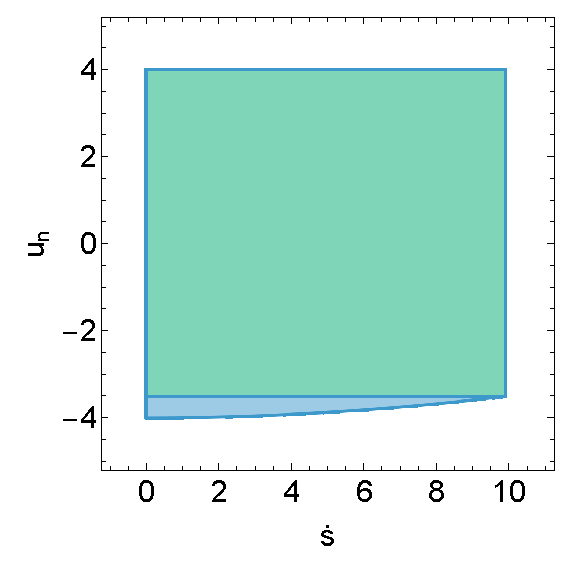
\includegraphics[width=\textwidth]{figures/inner_polytope/region_x3u2_plot_gr1.eps}
		\caption{Region $\dot{s}$ vs $u_n$}
	\end{subfigure}
	% Third image
	\begin{subfigure}[b]{0.32\textwidth}
		\centering
		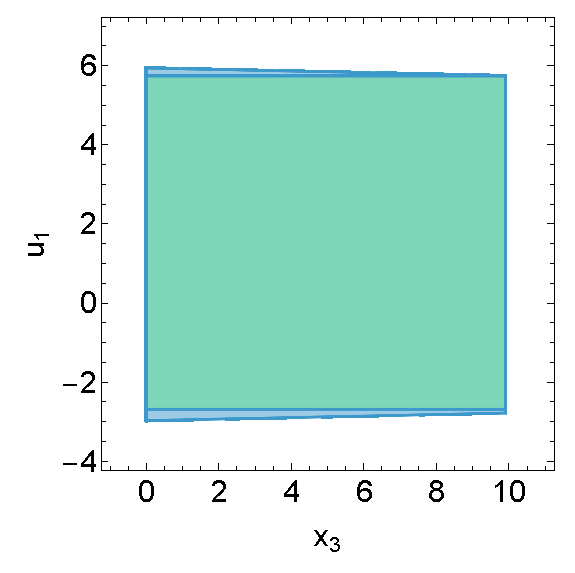
\includegraphics[width=\textwidth]{figures/inner_polytope/plot_gr1.eps}
		\caption{Region $u_t$ vs $u_n$}
	\end{subfigure}
	\caption{In Green using Interval Fitting \ref{subsubsec:interval_fitting} and in Blue using CAD \ref{subsubsec:cad}.}
	\label{fig:qe-comparison}
\end{figure}

In conclusion, eliminating the quantifiers with the first approach leads to a near-optimal result, comparable to the one achieved using the second
approach with CAD.
However, using CAD has a significant downside that we have not yet mentioned.
It is not guaranteed that the resulting formula is convex.
Typically, you will encounter disjunctions of polynomial inequalities, which cannot be handled by a convex solver without resorting to integer
programming or an equivalent approach.
It is also not guaranteed that each polynomial inequality follows the DCP rules, even if the set described by the resulting formula is convex.
Additional techniques would be required to use the second approach for our planner.

In cases where the resulting set is convex, we used a sampling approach to obtain an inner approximation described by half-spaces.
This results in a sequence of linear constraints that all must be satisfied, thus losing a small proportion of the original set.
Consequently, the difference between our first approach and the second approach becomes even smaller.
Additionally, we end up with double or triple the number of constraints on each state variable and each control input, which may lead to slower
solver times.

Overall, while the CAD approach provides a more accurate result, the first approach offers a good balance between computational efficiency and
accuracy, making it a viable option for practical applications.

\subsubsection{Limitations and Outlook}\label{subsubsec:limitations_and_outlook}

While the $\forall$-elimination approach provides a computationally efficient method to find intervals for the variables of interest, it can be quite restrictive for several reasons:

\begin{itemize}
	\item \textbf{Conservativeness:}
	      The approach tends to be conservative because it ensures that the constraints hold for all possible values within the intervals.
	      This often leads to smaller intervals, which may exclude feasible solutions that could be considered by less conservative methods.
	\item \textbf{Dependence on Affine Functions:}
	      The first method relies on the assumption that the function $f(x, y)$ is affine in $x$ and all variables in $y$ are bounded.
	      If this assumption does not hold, the approach may not be applicable.
\end{itemize}

Overall, while the $\forall$-elimination approach is useful for its simplicity and computational efficiency, it may lead to overly restrictive
solutions that do not fully exploit the feasible region.

Consider a scenario with a tight turn followed by a long straight road.
In such cases, the model will restrict $\dot{s}$ to an interval that is valid for both the tight turn and the straight road.
Consequently, the model will find a solution, but it will not be able to drive fast on the straight road, even though it is possible to drive faster
on the straight road than on the tight turn.

To address this issue, we can introduce segments of the road, one for the straight road and one for the tight turn.
We can independently construct the coupling constraints set for each segment.
However, this introduces a new problem: how to switch between the segments.
Our solution involves using the current vehicle velocity to predict when the vehicle will reach the end of the segment.
Knowing the vehicle's current position, velocity, and the distance to the end of the segment, we can calculate the time it will take to reach the
end.

Further, both approaches do not consider the possibility of achieving a larger feasible set by restricting $\dot{n}$ to a smaller interval.
The first approach handles the problem by using the bounds on $s$, $n$, and $\dot{n}$ to find the intervals for $\dot{s}$, which are then used for
$u_t$ and finally for $u_n$.
However, changing the order may lead to better results for desired driving behavior.

Given the simplicity of the first approach, we implemented a non-linear program that defines the relationships between the intervals with variables
as upper and lower bounds.
By adding constraints, we can define an objective that models certain driving behaviors.
For example, one might want to be able to slow down as quickly as possible or maximize the upper speed limit.
The latter objective leads to the following intervals:

\begin{figure}[h]
	\centering
	\begin{subfigure}[b]{0.45\textwidth}
		\centering
		\begin{align*}
			0    & \leq s \leq 10       \\
			0    & \leq n \leq 2        \\
			0    & \leq \dot{s} \leq 10 \\
			-2   & \leq \dot{n} \leq 2  \\
			-2.9 & \leq u_t \leq 5.9    \\
			-4   & \leq u_n \leq 3.75
		\end{align*}
		\caption{Initial Approach}
	\end{subfigure}
	\hfill
	\begin{subfigure}[b]{0.45\textwidth}
		\centering
		\begin{align*}
			0      & \leq s \leq 10,         \\
			0      & \leq n \leq 2,          \\
			0      & \leq \dot{s} \leq 10.05 \\
			-2     & \leq \dot{n} \leq 2     \\
			-2.899 & \leq u_t \leq 5.929     \\
			-4     & \leq u_n \leq 3.746
		\end{align*}
		\caption{Using Non-Linear Programming}
	\end{subfigure}
	\caption{Comparison of two sets of intervals for state variables and control inputs.}
\end{figure}

As you can see, the intervals on the right are preferable, as they only slightly reduce longitudinal acceleration while allowing for higher speeds.

In conclusion, we have successfully developed our first vehicle model for motion planning that can be solved using a convex solver.
Next, we will introduce a transformation that maps the state variables and control inputs of the planning model to a steering angle, which can be
used to control a vehicle based on the equations from \cite{eilbrecht_challenges_2020}.
A similar approach is demonstrated in \cite{werling_optimal_2010}, which served as an additional inspiration.


\subsection{Determining the Steering Angle} \label{subsec:determining_the_steering_angle}

Typically, a vehicle is controlled through throttle, brakes, and a steering angle.
To incorporate these controls, we need to move away from visualizing our model as a box aligned with the road.
Instead, we will treat the model as a point and define its orientation based on its velocity.
We set $v_y = 0$ and $a_y=0$ to reflect that lateral motion arises solely from steering, thereby keeping the lateral velocity state zero and
capturing lateral movement through changes in heading rather than a separate lateral speed.
Using the equations \eqref{eq:first_derivative_long} and \eqref{eq:first_derivative_lat} with $v_y = 0$, we can solve for $v_x$.
\begin{equation}
	v := v_x = \sqrt{(1-nC(s))^2\dot{s}^2 + \dot{n}^2}
\end{equation}
Dividing $\dot{n}$ by $\dot{s}$ combined with  \eqref{eq:first_derivative_long} and \eqref{eq:first_derivative_lat} yields:
\begin{equation}
	\frac{\dot{n}}{\dot{s}} = (1-nC(s))\tan(\xi) = (1-nC(s))\tan(\psi - \theta)
\end{equation}
which we can solve for $\psi$ to get the orientation of the vehicle.
\begin{equation}
	\psi = \theta + \arctan\left(\frac{\dot{n}}{\dot{s}(1-nC(s))}\right)
\end{equation}

Using the state variables and $g$ from \eqref{def:g}, we can calculate $a_{x,tn}$ and $a_{y,tn}$ from \eqref{def:axtn} and \eqref{def:aytn},
respectively.
By substituting these values into equations \eqref{eq:second_derivative_long} and \eqref{eq:second_derivative_lat}, and setting $a_y = 0$, we can
determine the longitudinal acceleration and the change in orientation.
Additionally, we assume $|\xi| \leq \frac{\pi}{2}$ to ensure that $\cos{\xi} \neq 0$.
\begin{align}
	\dot{\psi} = \frac{a_{y,tn} - \tan(\xi) a_{x,tn}}{v (\tan(\xi) \sin(\xi) + \cos(\xi))} \\
	a := a_x = \frac{a_{x,tn} + v \dot{\psi} \sin(\xi)}{\cos{\xi}}
\end{align}
Our bicycle models \eqref{eq:dpsi_steering_angle} enables us to calculate the steering angle.
\begin{equation}
	\delta = \arctan(l_{wb}\frac{\dot{\psi}}{v})
\end{equation}
With those equations, we can define a transformation.
\begin{equation}
	T(\tilde{x}_{di}, \tilde{u}_{di}) = [p_x, p_y, \psi, \dot{\psi}, v, a, \delta] \label{eq:pm_state_transformation} \end{equation}

\subsection{Exact Discretization of the Double Integrator Model}

Using the simplified state and control representation from
Section~\ref{subsubsec:resulting_simplified_model}, the system dynamics \eqref{eq:pm_final_dynamics} are discretized using the matrix exponential
method \cite{kailath_linear_1980, ogata_modern_2010}.
The discrete-time system is formulated as:

\begin{equation}
	\label{eq:discrete_time_dynamics_di}
	\tilde{x}_{di, k+1} = A_d \tilde{x}_{di, k} + B_d \tilde{u}_{di, k} =: f_{d, di}(\tilde{x}_{di, k}, \tilde{u}_{di, k}, \Delta t),
\end{equation}

where the exact discretization is given by:

\begin{equation}
	A_d = e^{A \Delta t}, \quad B_d = \left( \int_0^{\Delta t} e^{A \tau} d\tau \right) B.
\end{equation}

Using the closed-form solution for the matrix exponential \cite{noauthor_matrix_nodate}, we obtain:

\begin{equation}
	A_d = \begin{bmatrix}
		1 & 0 & \Delta t & 0        \\
		0 & 1 & 0        & \Delta t \\
		0 & 0 & 1        & 0        \\
		0 & 0 & 0        & 1
	\end{bmatrix},
	\quad
	B_d = \begin{bmatrix}
		\frac{\Delta t^2}{2} & 0                    \\
		0                    & \frac{\Delta t^2}{2} \\
		\Delta t             & 0                    \\
		0                    & \Delta t
	\end{bmatrix}.
\end{equation}

This formulation ensures that the discrete-time representation accurately follows the continuous-time system over a sampling interval \( \Delta t \),
preserving dynamic consistency while enabling efficient convex optimization.
The resulting discrete-time model will be used in the subsequent trajectory planning formulation.

\subsection{Final Model Representation} \label{subsec:pm_resulting_model}

Our final model is represented by the following tuple.
\begin{equation}
	M_{pm} = (\tilde{x}_{di}, \tilde{u}_{di}, f_{d, di}, \hat{C}, T)
	\label{model:point_mass}
\end{equation}
